\section{Implementación}

\subsection{Requisitos y Tecnologías}

El desarrollo de \textbf{8-Track} se llevó a cabo en el lenguaje de programación \textbf{C++20} y contó con el
uso de múltiples dependencias del framework \textbf{Qt}.

\begin{table}[htbp]
	\centering
	\begin{tabularx}{\textwidth}{@{}llX@{}}
		\toprule
		Tecnología   & Versión     & Uso                        \\
		\midrule
		C++          & 20          & Lenguaje de implementación \\
		QtQuick      & Qt 6.8+     & Interfaz gráfica           \\
		QtSQL        & Qt 6.8+     & Acceso a la base de datos  \\
		QtMultimedia & Qt 6.8+     & Reproducción de audio      \\
		SQLite       & vía QSQLITE & Motor de base de datos     \\
		\bottomrule
	\end{tabularx}
	\caption{Tecnologías del núcleo de la aplicación}
\end{table}

Todas las dependencias \texttt{third-party} se descargan automáticamente antes de la compilación por medio
de \texttt{FetchContent}; por lo tanto, es necesario contar con conexión a internet.

\begin{table}[htbp]
	\centering
	\begin{tabularx}{\textwidth}{@{}llX@{}}
		\toprule
		Herramienta & Versión & Uso                                     \\
		\midrule
		CMake       & 3.25+   & Configuración y generación del proyecto \\
		Ninja       & ---     & Generador del preset de release         \\
		ccache      & ---     & Caché de compilación                    \\
		mold        & ---     & Enlazador del preset de release         \\
		\bottomrule
	\end{tabularx}
	\caption{Herramientas de construcción}
\end{table}

\begin{table}[htbp]
	\centering
	\begin{tabularx}{\textwidth}{@{}llX@{}}
		\toprule
		Biblioteca & Versión & Uso                                          \\
		\midrule
		TagLib     & 2.3.2   & Lectura de las etiquetas ID3v2.4 y carátulas \\
		PicoSHA2   & 1.0.1   & Hash para el caché de las carátulas          \\
		argparse   & 3.2     & Argumentos para la CLI                       \\
		tabulate   & 2.0     & Presentación de datos tabulados para la CLI  \\
		indicators & 2.3     & Barra de progreso para la CLI                \\
		\bottomrule
	\end{tabularx}
	\caption{Bibliotecas de terceros utilizadas por la aplicación}
\end{table}

\begin{table}[htbp]
	\centering
	\begin{tabularx}{\textwidth}{@{}llX@{}}
		\toprule
		Herramienta    & Versión & Uso                         \\
		\midrule
		GoogleTest     & 1.15.2  & Pruebas unitarias           \\
		prek           & 0.5     & Gestión de hooks de Git     \\
		clang-format   & 23.1.1  & Formato del código C++      \\
		qmlformat      & 1.2.0   & Formato del código QML      \\
		Doxygen        & 1.18    & Generación de documentación \\
		GitHub Actions & ---     & Integración continua (CI)   \\
		\bottomrule
	\end{tabularx}
	\caption{Herramientas de pruebas, calidad y documentación}
\end{table}

\subsection{Instrucciones de Compilación}

Se recomienda utilizar el preset \texttt{release}, que centraliza la
configuración empleada durante el desarrollo y en integración continua.
Este utiliza Ninja para la construcción, ccache para reutilizar resultados
de compilaciones anteriores y mold para acelerar el enlazado.

Para utilizarlo, es necesario contar con estas herramientas instaladas.
En \textbf{Fedora}, pueden instalarse con el siguiente comando:

\begin{lstlisting}[language=bash]
sudo dnf install ninja-build mold ccache
\end{lstlisting}

Primero, se debe clonar el repositorio y acceder al directorio del proyecto:

\begin{lstlisting}[language=bash]
git clone https://github.com/evanrock520-ciencias/8-Track.git
cd 8-Track
\end{lstlisting}

A continuación, se puede elegir una de las siguientes alternativas.
Ambas compilan el proyecto en modo \texttt{Release}.

\paragraph{Compilación con preset}

El preset almacena los archivos generados en \texttt{build/release}:

\begin{lstlisting}[language=bash]
cmake -S . --preset release
cmake --build --preset release
\end{lstlisting}

\paragraph{Compilación sin preset}

Como alternativa, se puede configurar la construcción directamente,
sin exigir Ninja, ccache ni mold. En este caso, los archivos generados
se almacenan en \texttt{build}:

\begin{lstlisting}[language=bash]
cmake -S . -B build -DCMAKE_BUILD_TYPE=Release
cmake --build build
\end{lstlisting}

\subsection{Instrucciones de Ejecución}

\subsubsection*{Interfaz Gráfica}

En el primer arranque, la aplicación crea automáticamente la base de datos SQLite e inicializa su esquema. Los datos se
almacenan en el directorio determinado por \texttt{QStandardPaths::AppDataLocation}, que en Linux normalmente corresponde
a \texttt{\$HOME/.local/share/8-track/}

\paragraph{Abrir interfaz gráfica}

\begin{lstlisting}[language=bash]
build/release/8-track/qml/track8
\end{lstlisting}

La biblioteca inicialmente está vacía. Para agregar canciones se debe seleccionar un directorio mediante el botón \texttt{Scan}
de la interfaz gráfica o mediante el comando \texttt{--scan} de la CLI.

Al seleccionar el directorio, comienza el escaneo de los archivos MP3
y se muestra una ventana con el progreso y el archivo actual.

\begin{center}
	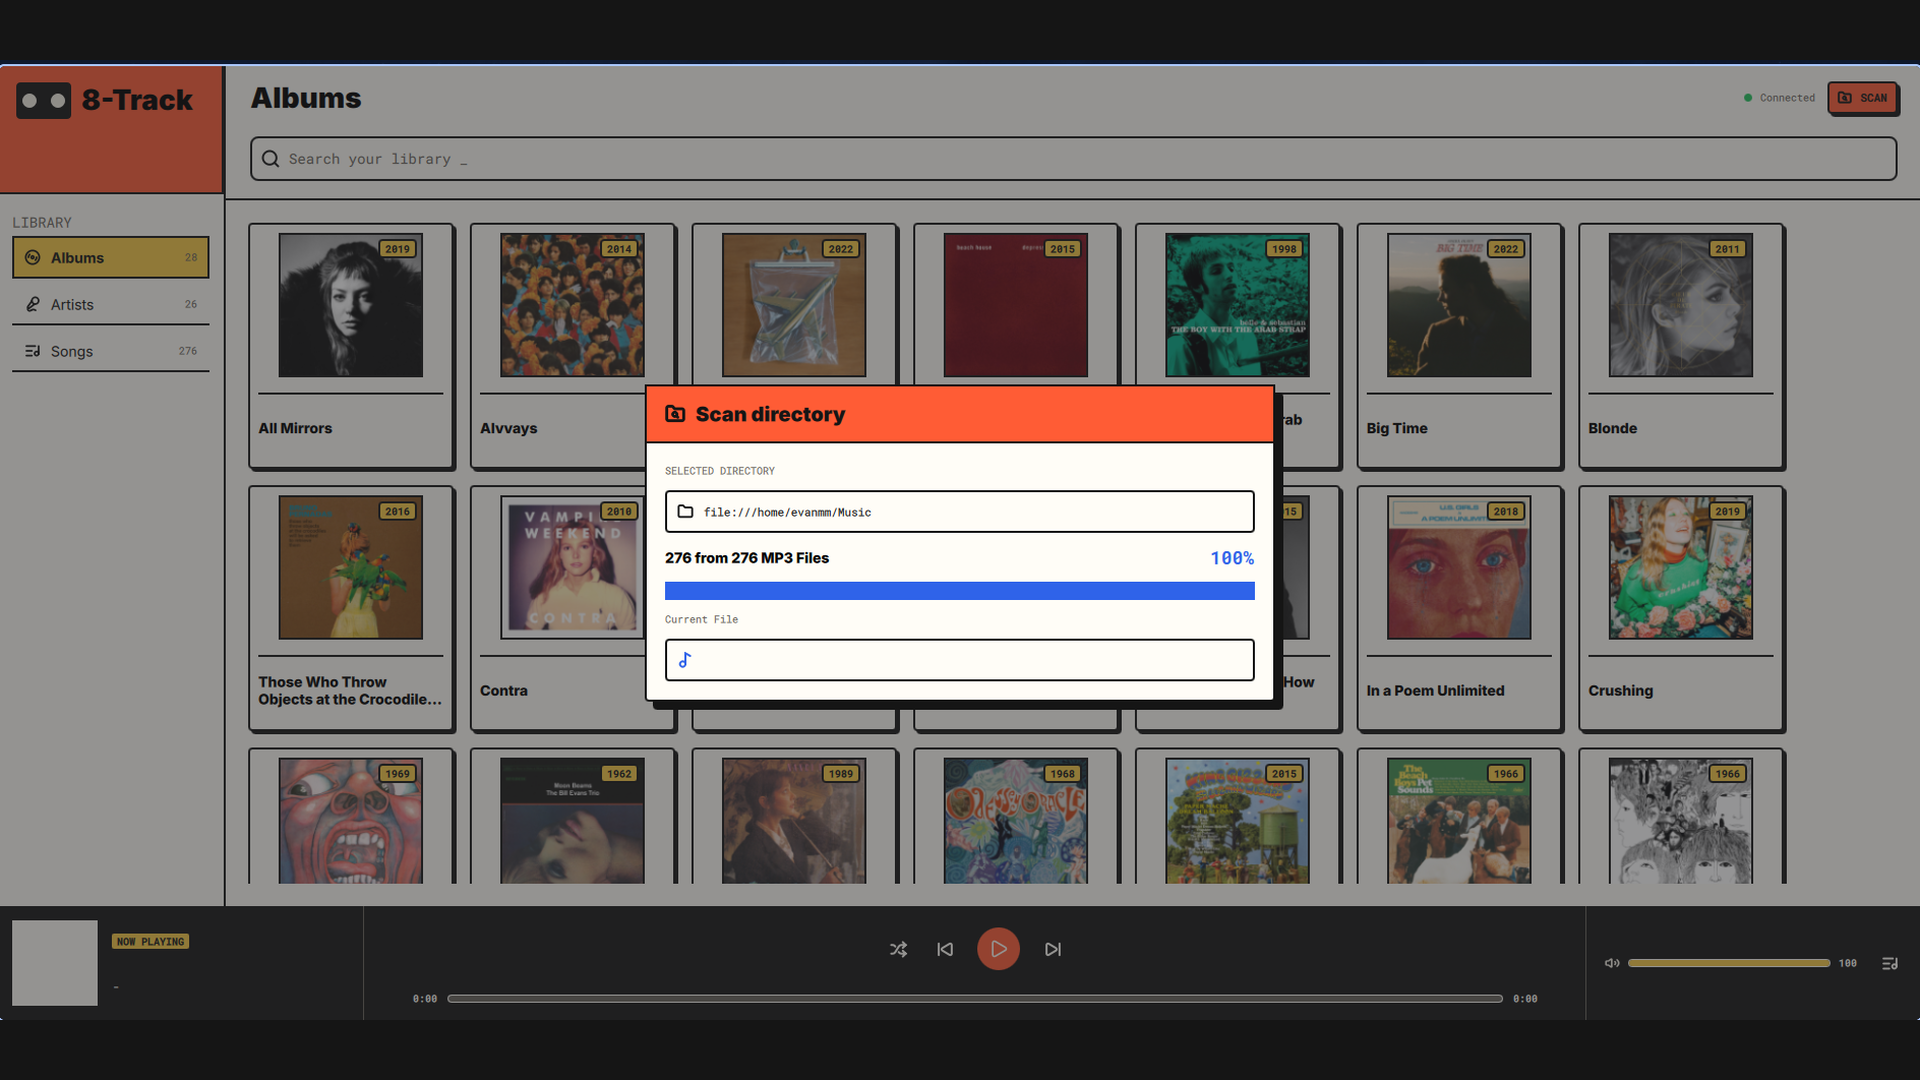
\includegraphics[width=0.8\linewidth,trim=0bp 60bp 0bp 60bp,clip]{screnshoots/scan.png}
\end{center}

Al finalizar, la biblioteca se actualiza con las canciones,
álbumes e intérpretes encontrados.

\begin{center}
	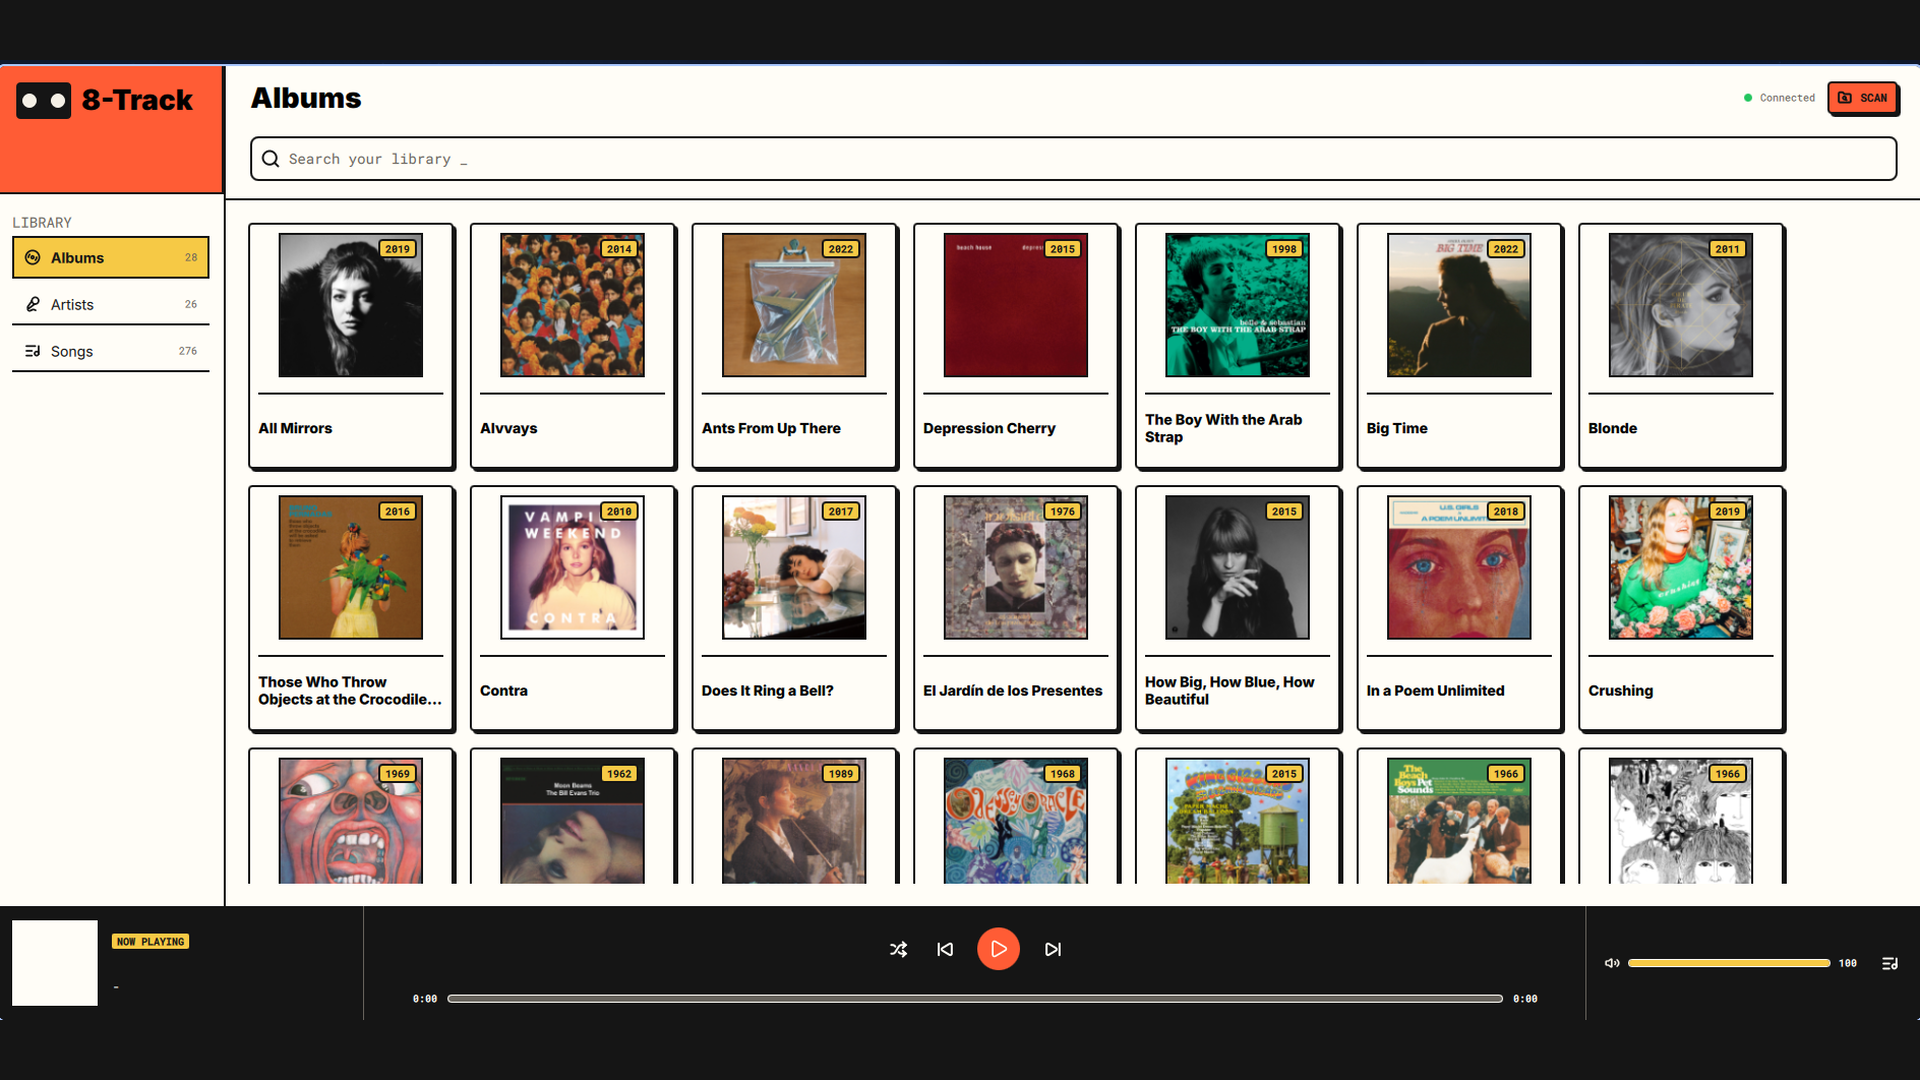
\includegraphics[width=0.8\linewidth,trim=0bp 60bp 0bp 60bp,clip]{screnshoots/landing.png}
\end{center}

Para iniciar la reproducción, se utiliza el botón de reproducción de una canción o de un álbum. La barra
inferior permite pausar o reanudar el audio, cambiar de canción, activar el modo aleatorio y ajustar el
volumen y la posición de reproducción.

\begin{center}
	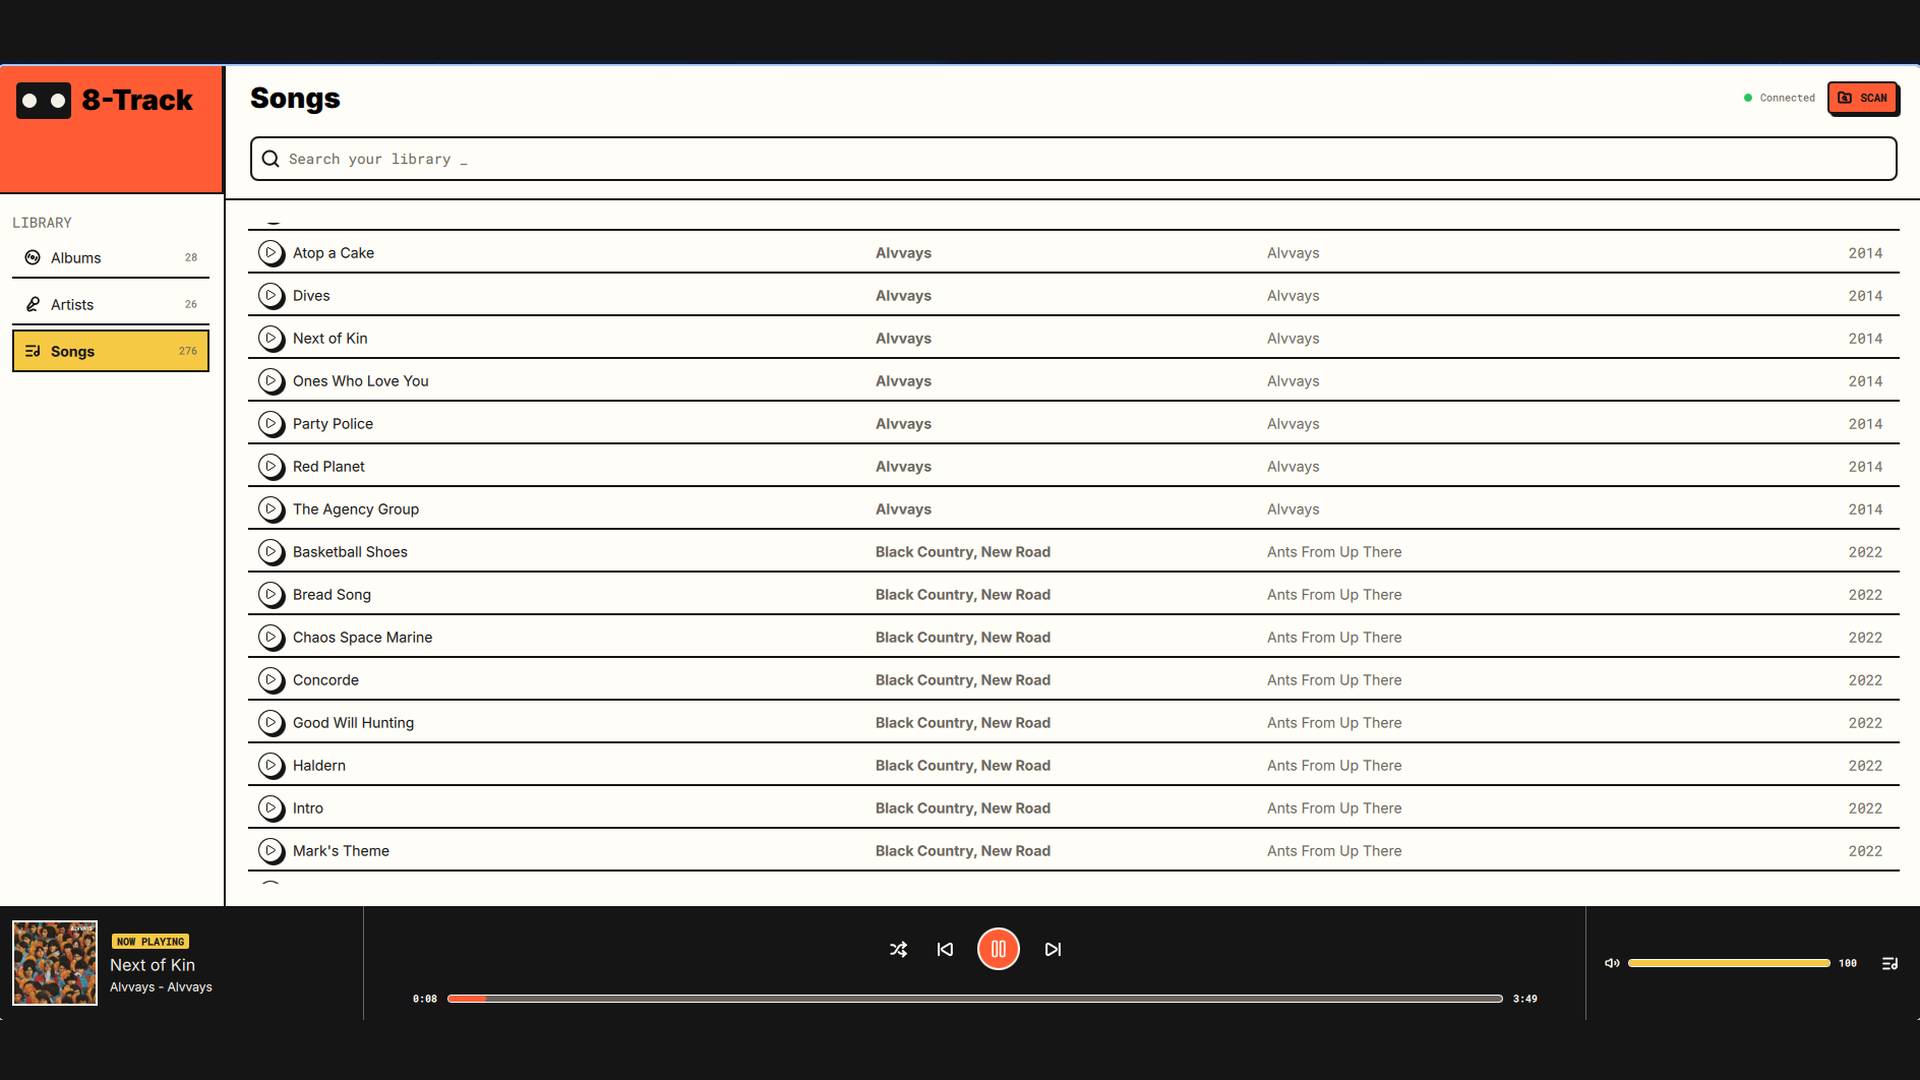
\includegraphics[width=0.8\linewidth,trim=0bp 60bp 0bp 60bp,clip]{screnshoots/playback.png}
\end{center}

Para buscar canciones, se escribe una consulta de MuQL en la barra superior y se presiona \texttt{Enter};

\begin{center}
	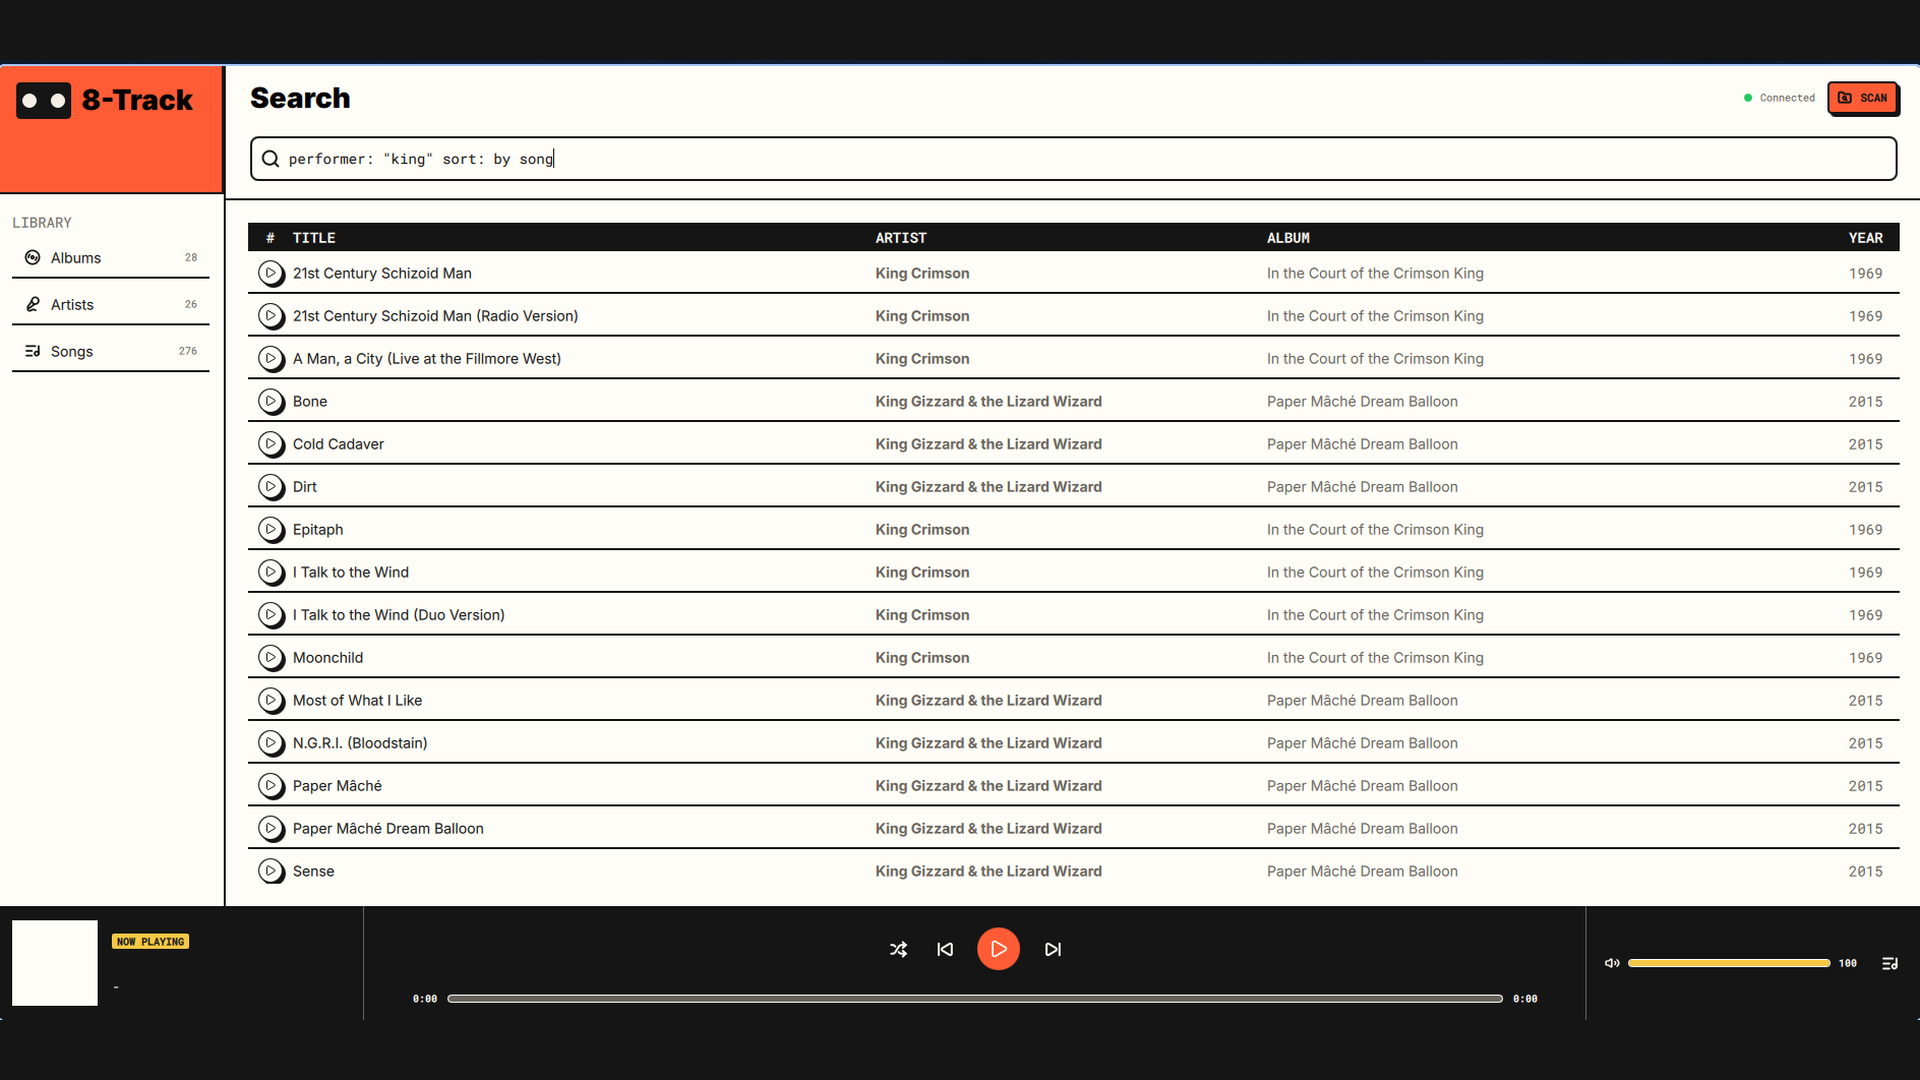
\includegraphics[width=0.8\linewidth,trim=0bp 60bp 0bp 60bp,clip]{screnshoots/search.png}
\end{center}

\subsubsection*{CLI}

\paragraph{Escanear un directorio}

\begin{lstlisting}[language=bash]
build/release/track8-cli --scan $HOME/Music
\end{lstlisting}

\paragraph{Ver la biblioteca}

\begin{lstlisting}[language=bash]
build/release/track8-cli --list
\end{lstlisting}

\begin{center}
	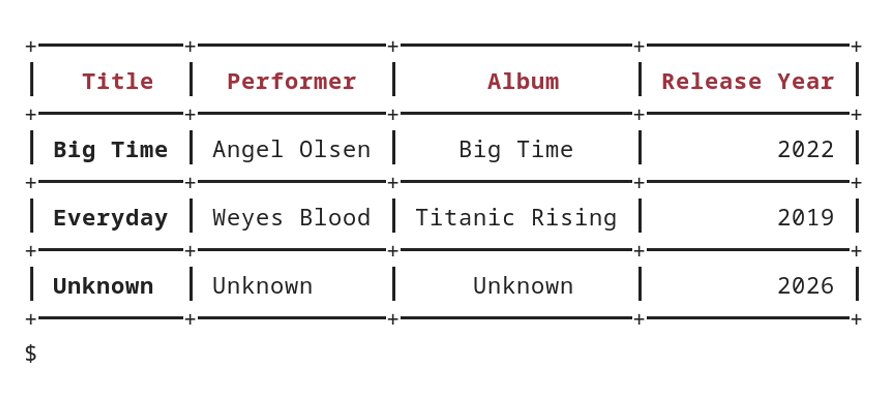
\includegraphics[width=0.68\textwidth,trim=16bp 68bp 16bp 30bp,clip]{screnshoots/library.png}
\end{center}

\paragraph{Realizar una consulta}

\begin{lstlisting}[language=bash]
build/release/track8-cli --query 'big'
\end{lstlisting}

\begin{center}
	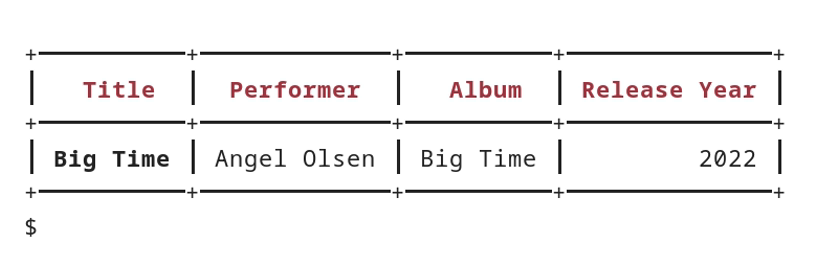
\includegraphics[width=0.62\textwidth,trim=16bp 70bp 48bp 40bp,clip]{screnshoots/query.png}
\end{center}

\subsection{Pruebas}

La mayoría del proceso de desarrollo fue guiado por pruebas unitarias desarrolladas con la biblioteca de \textbf{GoogleTest}.
Las pruebas están divididas por módulos, cada uno correspondiente a una biblioteca de \textbf{8-Track}.

\begin{table}[htbp]
	\centering
	\begin{tabularx}{\textwidth}{@{}lX@{}}
		\toprule
		Suite    & Cobertura                                                            \\
		\midrule
		database & Implementación de los repositorios para SQLite                       \\
		domain   & Validación de fechas                                                 \\
		compiler & Pruebas para lexer, parser, generación del AST y transpilación a SQL \\
		miner    & Mineria de metadatos con archivos de prueba heterogéneos             \\
		player   & Lógica de la cola de reproducción.                                   \\
		services & Verificación de datos y acciones de usuario                          \\
		\bottomrule
	\end{tabularx}
	\caption{Suites de pruebas unitarias}
\end{table}

\paragraph{Ejecutar Pruebas}

Para ejecutar todas las suites de pruebas registradas en CTest,
se utiliza el siguiente comando:

\begin{lstlisting}[language=bash]
ctest --test-dir build/release/ --output-on-failure
\end{lstlisting}

También es posible ejecutar una suite de pruebas de manera
individual, invocando directamente su ejecutable. Por ejemplo,
para ejecutar la suite correspondiente a la base de datos:

\begin{lstlisting}[language=bash]
./build/release/tests/database_tests
\end{lstlisting}

\subsection{CI/CD}

\subsubsection*{Verificación}

El \texttt{workflow} principal de \texttt{CI} sirve principalmente como una verificación de reproducibilidad
del sistema. Se encarga de configurar el entorno, descargar dependencias, verificar el formato de código,
compilar \textbf{8-Track} y correr las suites de pruebas unitarias.

\subsubsection*{Calidad}

La calidad, legibilidad y consistencia del código es bastante importante para mí.
Por ello, en lugar de depender de una disciplina manual para mantener un formato consistente, el proceso
se automatiza mediante \textit{hooks} de \texttt{prek}: \texttt{clang-format} para \textbf{C++} y
\texttt{qmlformat} para \textbf{QML}. Estos se ejecutan antes de cada \textit{commit} y se vuelven a verificar
en el \texttt{workflow} principal de \texttt{CI}, de modo que ningún cambio con formato inconsistente llega
a \texttt{main}.


\subsubsection*{Documentación}

Durante cada \texttt{push} a la rama \texttt{main} se ejecuta un despliegue automático de documentación
relacionada al código del proyecto en \url{https://evanrock520-ciencias.github.io/8-Track/}.
